% \documentclass{article}
% \usepackage[dvipsnames]{xcolor}
% \usepackage{tikz}
% \usepackage{xcolor,colortbl}
% 
% \begin{document}
% 
% \newcommand{\gringo}{\textit{gringo}}
\newcommand{\clasp}{\textit{clasp}}
\newcommand{\clingo}{\textit{clingo}}
\newcommand{\asprin}{\textit{asprin}}
\newcommand{\asap}{\textit{teaspoon}}
\newcommand{\piclasp}{\textit{piclasp}}

\newcommand{\code}[1]{\lstinline[basicstyle=\ttfamily]{#1}}

\newcommand{\lw}[1]{\smash{\lower1.ex\hbox{#1}}}
\newcommand{\llw}[1]{\smash{\lower3.ex\hbox{#1}}}

%\newcommand{\dataCL}[5]{%
%  \code{#1} & #3 & #5 & #4
%}
%\newcommand{\dataCS}[5]{%
%  #3 & #5 & #4
%}

\newenvironment{tableC}{%
  \scriptsize
  \tabcolsep = 0.6mm
  \begin{tabular}[t]{l|rlr|rlr|rlr|rlr|rlr}\hline
    \multicolumn{1}{l|}{\llw{Instance}} &
    \multicolumn{3}{c|}{UD1} &
    \multicolumn{3}{c|}{UD2} &
    \multicolumn{3}{c|}{UD3} &
    \multicolumn{3}{c|}{UD4} &
    \multicolumn{3}{c}{UD5} \\
    & 
    \multicolumn{1}{c}{Best} & & \multicolumn{1}{c|}{\emph{tea-}} & 
    \multicolumn{1}{c}{Best} & & \multicolumn{1}{c|}{\emph{tea-}} & 
    \multicolumn{1}{c}{Best} & & \multicolumn{1}{c|}{\emph{tea-}} & 
    \multicolumn{1}{c}{Best} & & \multicolumn{1}{c|}{\emph{tea-}} & 
    \multicolumn{1}{c}{Best} & & \multicolumn{1}{c}{\emph{tea-}} \\
    & 
    known & & \emph{spoon} & 
    known & & \emph{spoon} & 
    known & & \emph{spoon} & 
    known & & \emph{spoon} & 
    known & & \emph{spoon} \\
    \hline
  }{%
    \hline
  \end{tabular}
}

\newenvironment{tableB}{%
  \scriptsize
  \tabcolsep = 0.7mm
%  \begin{tabular}[t]{|l|c|r|l|l|l|}\hline
  \begin{tabular}[t]{lcrlll}\hline
    Instance &
    Formulation &
    Time (sec.)\\
    \hline
  }{%
    \hline
  \end{tabular}
}
\newenvironment{tableL}{%
  \scriptsize
  \tabcolsep = 0.7mm
  \begin{tabular}[t]{l|rrrrrrrr|r}\hline
    \lw{Instance} &
    \lw{Time (sec.)} &
    \multicolumn{6}{c}{The best utility vector} &
    The sum of  &
    The best of basic\\
    &
    &
    $(S_1,$ & $S_4,$ & $S_2,$ & $S_7,$ & $S_6,$ & $S_3)$ &
    utility vector &
    and optimized \\
    \hline
  }{%
    \hline
  \end{tabular}
}

%%% Local Variables:
%%% mode: latex
%%% TeX-master: "paper"
%%% End:


% \begin{figure}[t]
%   \centering

    \usetikzlibrary{shapes.misc, positioning}
    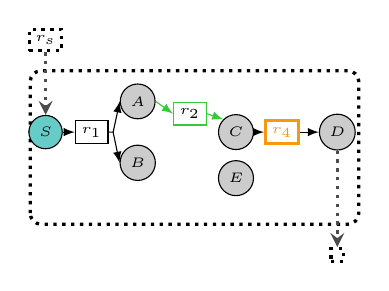
\begin{tikzpicture}[scale=0.39]\tiny
      \tikzstyle{metabolite}=[draw,circle,fill=white!80!black];
      \tikzstyle{repairmetabolite}=[draw,white!40!black, circle,fill=white!90!black,text=white!40!black,dashed];
      \tikzstyle{seed}=[draw,circle,fill=BlueGreen!70];%white!80!black
      \tikzstyle{target}=[draw,circle,fill=YellowOrange];%white!40!black
      \tikzstyle{reaction}=[draw,rectangle];
       \tikzstyle{export}=[draw,rectangle,dotted, very thick];
       \tikzstyle{exportrepair}=[draw,rectangle,dotted, very thick,white!80!black,text=white!70!black];
      \tikzstyle{repairreaction}=[draw,rectangle,white!40!black,text=white!40!black,dashed];
      \tikzstyle{solreaction}=[draw,rectangle,LimeGreen,text=black];
      \tikzstyle{initial}=[->,>=latex,thick];
      \tikzstyle{bdd}=[->,>=latex,thick];
      \tikzstyle{etiq}=[midway,fill=black!20,scale=0.5];
      \tikzstyle{stc}=[draw, rectangle, white, text=black]


      \draw [black,dotted, rounded corners, very thick] (-0.5,4) rectangle (10.2,9);
     % \node (system) [draw, rounded rectangle] at (0,0) {} (7cm,5cm);

      \node[seed] (S) at (0,7) {$S$};
      \node[metabolite] (A) at (3,8) {$A$};
      \node[metabolite] (B) at (3,6) {$B$};
      \node[metabolite] (C) at (6.2,7) {$C$};
      \node[metabolite] (D) at (9.5,7) {$D$};
      \node[metabolite] (E) at (6.2,5.5) {$E$};

      \node[reaction] (R1) at (1.5,7) {$r_{1}$};
      \node[reaction, very thick,YellowOrange] (R4) at (7.7,7) {$r_{4}$}; %LimeGreen
      \node[solreaction] (R2) at (4.7,7.6) {$r_{2}$};
      %\node[solreaction] (R3) at (4.7,6.4) {$r_{3}$};

      % R1 : S => A + B
      \draw[->,>=latex] (S.east) -- (R1.west);
      \draw[->,>=latex] (R1.east) -- (2.2,7) -- (A.west);
      \draw[->,>=latex] (2.2,7)  -- (B.west);

      % R2 : A => C
      \draw[->,>=latex,LimeGreen] (A.east) -- (R2.west);
      \draw[->,>=latex,LimeGreen] (R2.east) -- (C.north west);

      % R3 : B => C + E
      %\draw[->,>=latex,LimeGreen] (B.east) -- (R3.west);
      %\draw[->,>=latex,LimeGreen] (R3.east) -- (C.south west);
      %\draw[->,>=latex,LimeGreen] (R3.east) -- (E.west);

      % R4 : C => D
      \draw[->,>=latex] (C.east) -- (R4.west);
      \draw[->,>=latex] (R4.east) -- (D.west);

      %export G
      \node[export] (outD) at (9.5,3) {\ExportReaction};
      \draw[->,>=stealth,white!30!black,dotted, very thick] (D.south) --  (outD.north);

      %import S2
      \node[export] (inS) at (0,10) {$r_{s}$};
      \draw[->,>=stealth,white!30!black,dotted, very thick] (inS) --  (S.north);

  \end{tikzpicture}
% \end{figure}

% \end{document}
